\subsection{Right-Handed Neutrinos}

Neutrinos having non-zero mass suggests the need of a finer physical description, or extension of the SM. Non-zero mass enables the existence of right-handed neutrinos and left-handed anti-neutrinos, since they do not move at the speed of light. Yet all neutrinos have been observed with left-handed and all anti-neutrinos right-handed chirality --- a relativistic invariant of any particle. A key unanswered question in particle physics is: can neutrinos and anti-neutrinos be differentiated just by their chirality, or do right-handed neutrinos and left-handed anti-neutrinos exist as separate particles? \\

\subsection{The $\nu$MSM}


One possible extension to the Standard Model is the addition of $3$ right-handed neutrinos. Dubbed the $\nu$MSM, it was originally proposed by \cite{nuMSM_1, nuMSM_2}. Such right-handed neutrinos would have no electric charge, no lepton charge, and no color, making them insensitive to all fundamental interactions aside from gravity, making them particularily challenging to detect. As such, they are often refered to as \textbf{sterile neutrinos} ($\nu_s = \nu_{\textsc{i}, \textsc{ii}, \textsc{iii}}$) to distinguish them from their left-handed lepton-flavoured counterparts ($\nu_\ell = \nu_{e, \mu, \tau}$). Fig.~\ref{fig:numsm} recaps these additions to the SM picture. \\

\begin{figure}[h]
\begin{center}
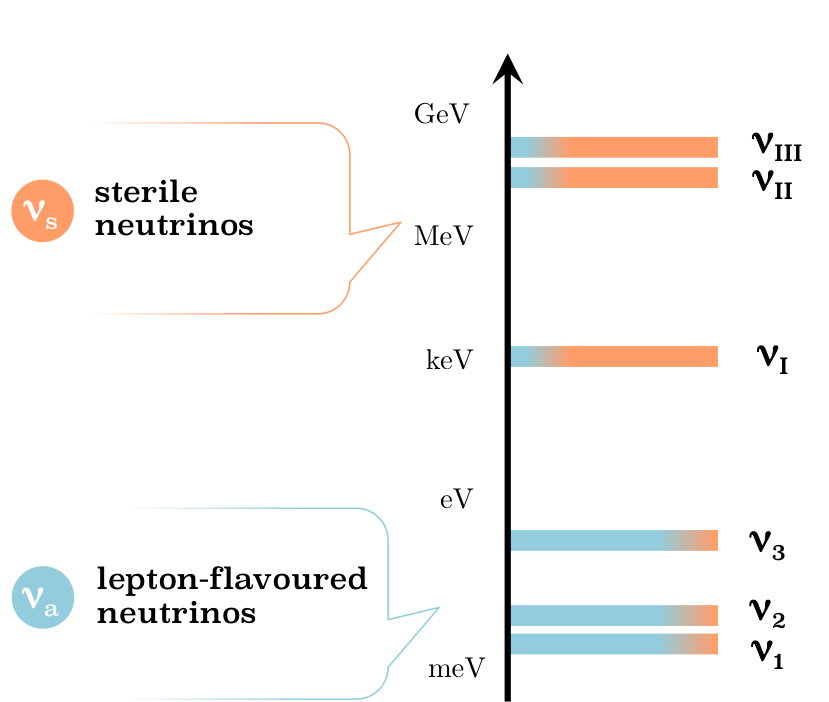
\includegraphics[width=0.5\columnwidth]{Neutrino/activesterile.png}
\caption{Assuming there are $3$ additional mass eigenstates $\nu_{\textsc{i}, \textsc{ii}, \textsc{iii}}$ such that $m_{\textsc{i}, \textsc{ii}, \textsc{iii}} \gg m_{1,2,3}$, and the angle between these heavier and lighter states is small, then the lepton-flavoured left-handed neutrinos of the SM can be thought of as a mixture of preponderantly the lighter eigenstatestates; whereas the $3$ remaining neutrinos are predominantly of the heavier eigenstates, carry no lepton flavour and are right-handed.}
\label{fig:actster}
\end{center}
\end{figure}


There are no theoretical limitations as to the scale of their rest mass, which can span from sub-eV to several $10^{15}$ GeV \citep{Drewes_nus}. If, however, the masses are of and above the GeV scale for at least two of the sterile neutrinos, and of the keV scale for the remaining one, then the $\nu$MSM is a particularily attractive model in that it provides a theoretical framework to simultaneously explain\\

\begin{itemize}
\item[$\bullet$] how neutrinos can get their mass without the Higgs mechanism, through a mechanism called a \textit{seesaw};\\
\item[$\bullet$] account for CP violation and the production of more leptons than antileptons (net global lepton asymmetry); \\
\item[$\bullet$] a candidate particle for the dark matter component of the Universe's energy density. \\
\end{itemize} 

The first two are beyond the scope of this work. In this thesis, I investigate whether the $\sim$keV sterile neutrino is a viable dark matter candidate particle. \\


\subsection{Experimental Searches}

One way to detect such a right-handed neutrino is indirectly through the products of its decay into a photon and a left-handed neutrino:

\begin{equation}
\begin{array}{lcr}
\nu_s & \longrightarrow & \nu_\ell + \gamma
\end{array}
\end{equation} \\ The decay products acquire a momentum of $\sim m_{\nu_s}/2$ where $m_{\nu_s}$ is the mass of the sterile neutrino. X-ray signatures in sterile neutrino rich systems would provide evidence for the decay of an $m_{\nu_s} \sim \mathrm{keV}$ sterile neutrino. \\

In the $\nu$MSM, the heavier neutrinos can be produced in the early Universe via oscillations with the lighter lepton-charged neutrinos. If one considers the $\nu_{1,2}$ mass eigenstates in Eq.~\ref{eq:2eigen} as a light ($\sim$eV) and a heavy ($\sim$keV) eigenstate, and replace $\nu_{e, \mu}$ with either a lepton-charged or sterile state $\nu_{\ell, s}$, then one can regard the $\theta_{12}$ angle as the angle between the light and heavy states. If $m_{2} \gg m_{1}$, as is assumed to be the case, then $\theta_{12} \ll 1$ as so is the probability of a lepton-charged state to oscillate into a sterile one $P \left( \nu_\ll \rightarrow \nu_s \right) \propto \sin^2 2 \theta_{12} \ll 1$. The diagonal elements of the Eq.~\ref{eq:2eigen} mixing matrix are close to 1. In laymen terms, the sterile states occupy nearly all of the heavy mass eigenstate while the neutrinos involved in weak interactions are principally made up of the lighter eigenstate and share very little of the heavy one. The half-life of a hypothetical sterile neutrino in this context is a function of the active-sterile mixing angle $\theta$. Detecting X-ray photons from sterile neutrino rich sources would therefore also provide a measurement of the mixing angle, assuming $m_{1,2,3} \ll m_{\textsc{i}, \textsc{ii}, \textsc{iii}}$. \\

If right-handed neutrinos can be produced via oscillations from weak-sensitive to weak-insensitive states, then a deficit in lepton-charged neutrinos is expected, however small. Thus far, the only tentative evidence for sterile neutrinos comes from an unaccounted for deficit of reactor neutrinos in \cite{Anomaly}, called the reactor anomaly. If, like the solar neutrino anomaly of the 1960s, it can be conclusively shown that these deficits are caused by oscillations from an active to a sterile state, then it would be an indirect evidence for the existence of sterile neutrinos. However, given their momentum and length on which these active-sterile oscillations would occur, the reactor anomalies would suggest sterile neutrino masses of a few eV. 

\begin{figure}
\begin{center}
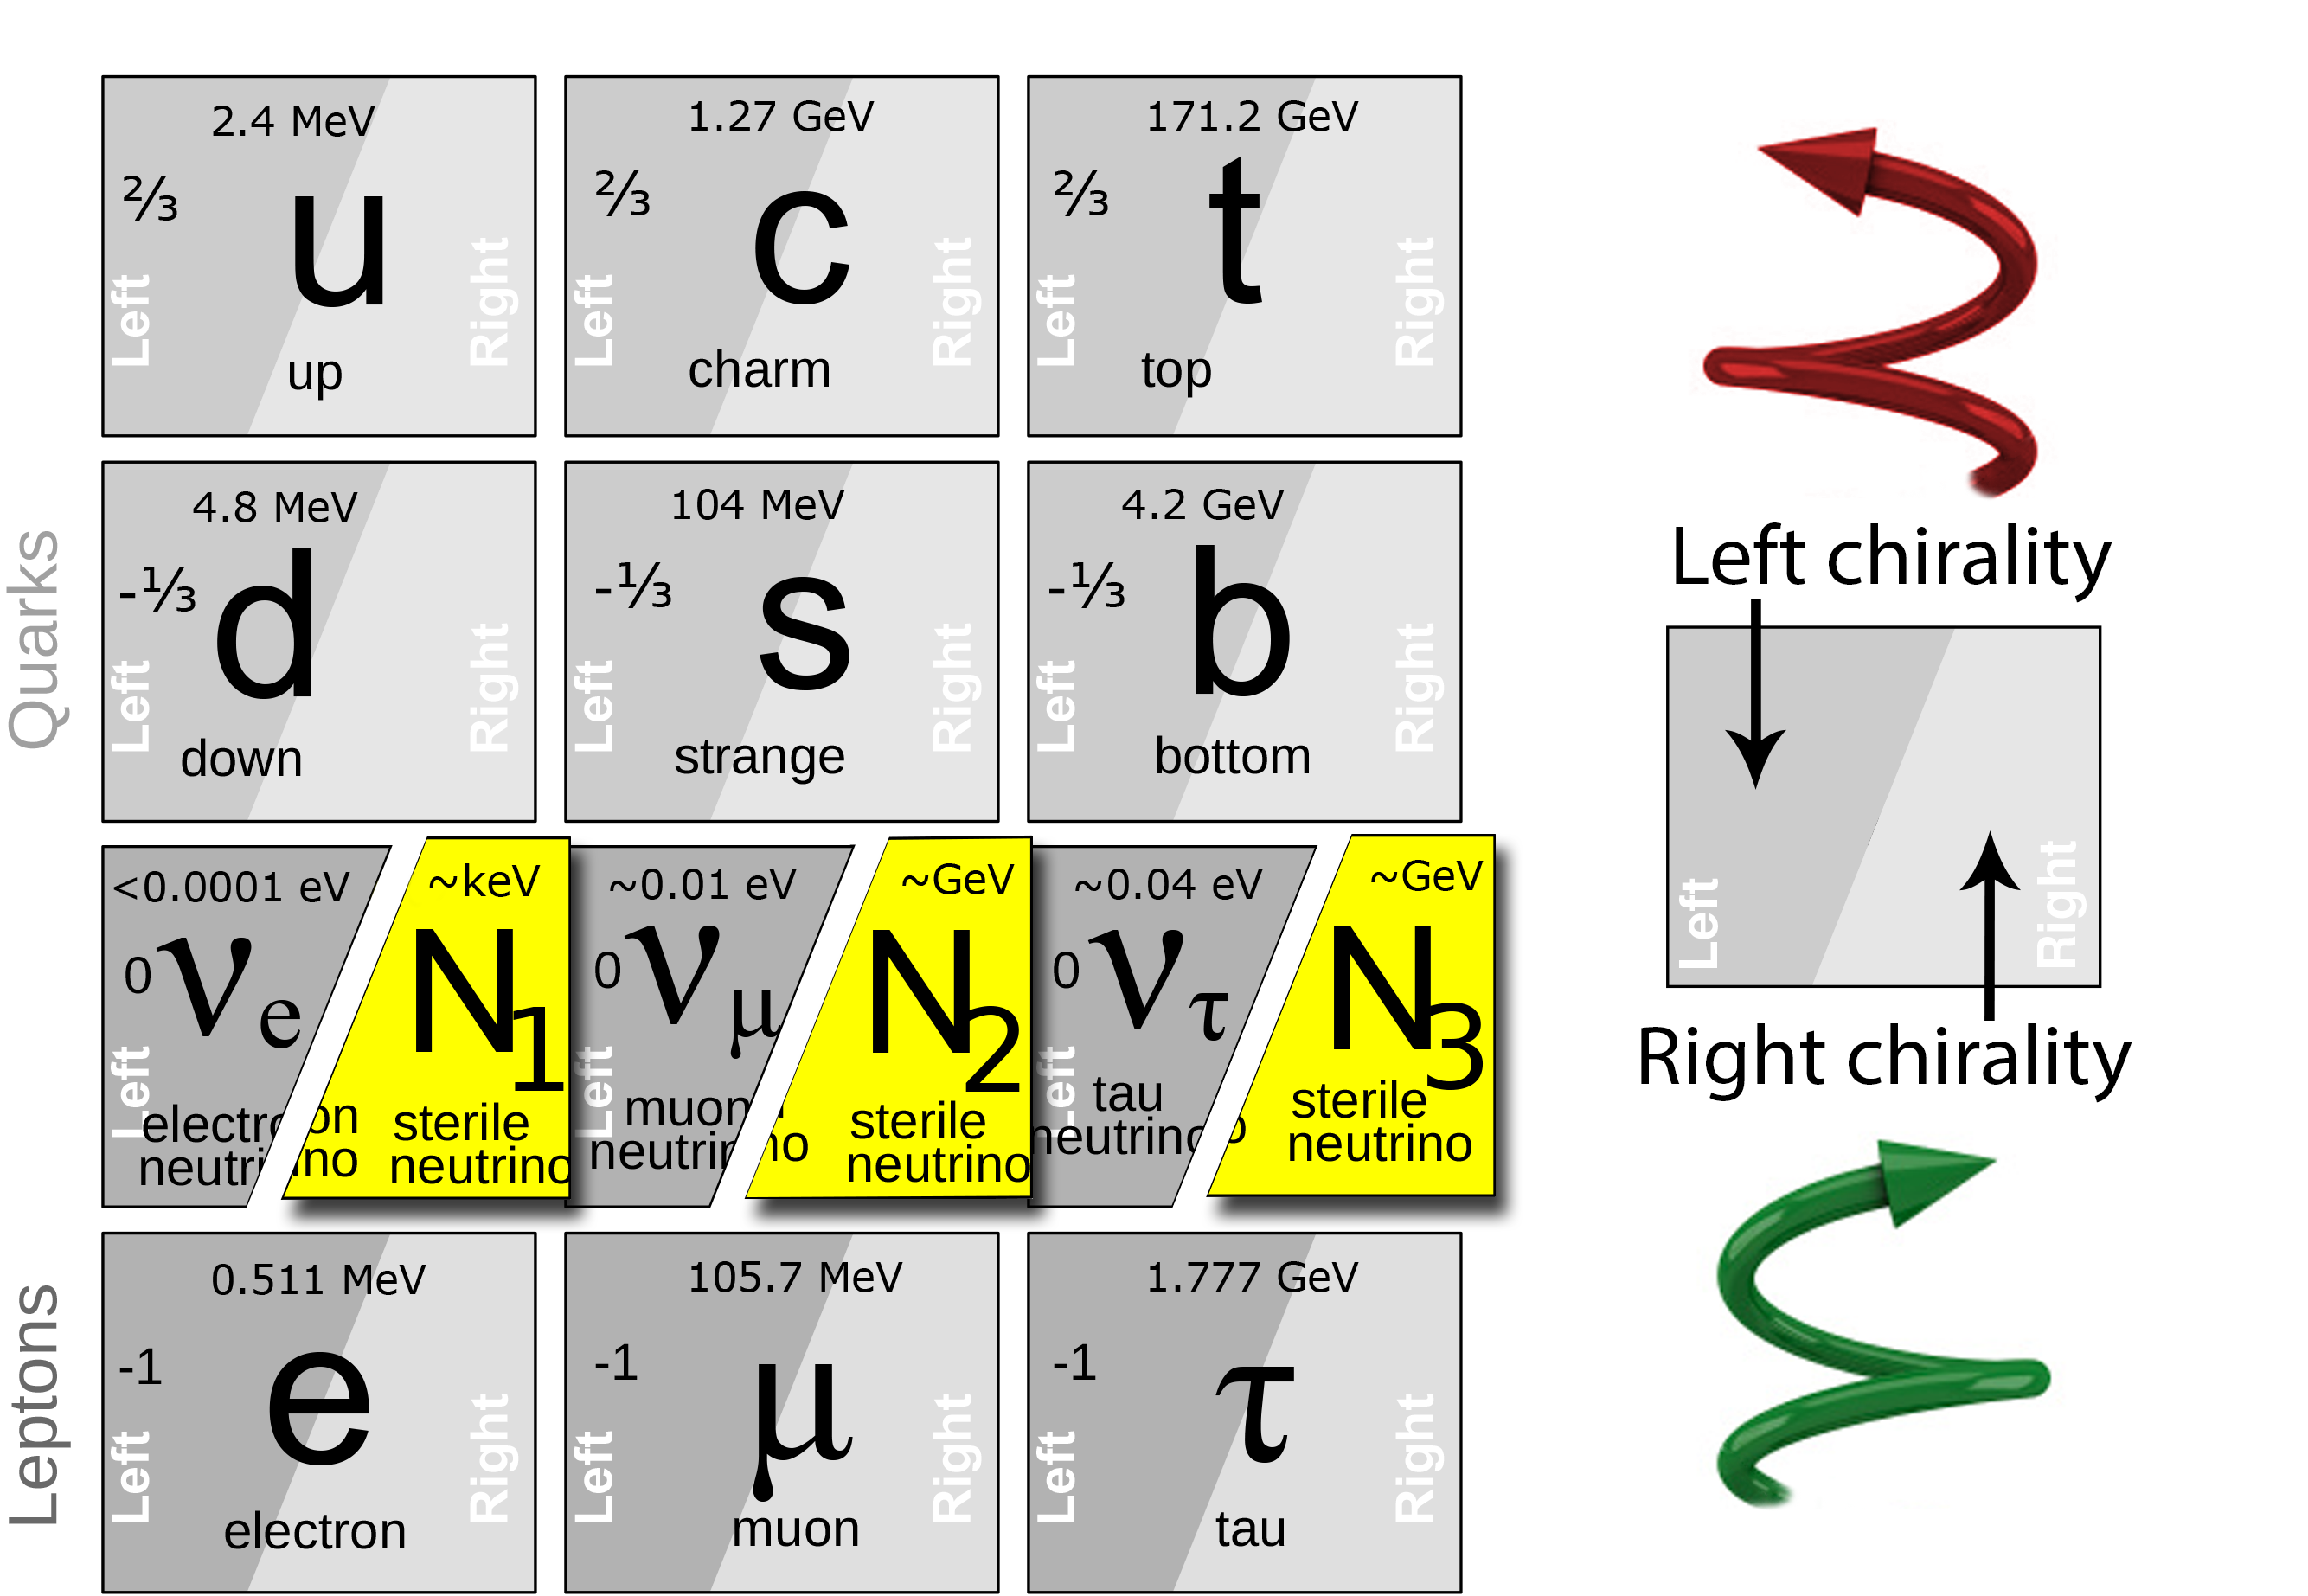
\includegraphics[width=0.8\columnwidth]{numsm.png}
\caption{Table comprising all fermions ($s/\hbar=1/2$) in the $\nu$MSM. The number in the top (\textit{resp.} left-side) of each panel is the particle's mass (\textit{resp.} electric charge). The only right chirality neutrinos in the SM are antineutrinos. In the $\nu$MSM, each of the lepton neutrinos has a heavy right-handed partner that has no lepton charge, in yellow. Credit: Alexey Boyarsky.}
\label{fig:numsm}
\end{center}
\end{figure}
